\section{Auswertung}
\label{sec:Auswertung}

\subsection{Bestimmung des effektiven Dämpfungswiederstand $R_{eff}$ und der Abklingdauer $T_{ex}$}
  Die bauteilspeziefischen Werte lauten:
  \begin{align*}
    L=12.78 \pm 0.09 \ mH\\
    C=2.066 \pm 0.006 \ nF\\
    R_1=67,2 \pm 0.2 \SI{1}{\ohm}\\
    R_2=682 \pm 1 \SI{1}{\ohm}
  \end{align*}
  Die gemessenen Extrema nach einem elektrischhen Nadelimpuls sind in der folgenden Tabelle aufgelisted.
  \begin{table}[H]
    \centering
    \caption{Ausgangswerte}
    \label{tab:data}
    \begin{tabular}{c c}
      \toprule
      Zeit [sec] & Spannung [V]\\
      \midrule
      0   & -10  \\
      13  & 17  \\
      26  & -8  \\
      40  & 13  \\
      52  & -5  \\
      68  & 10  \\
      81  & -3  \\
      95  & 9  \\
      110 & 0  \\
      120 & 7  \\
      132 & 1  \\
      147 & 6.5  \\
      162 & 2  \\
      175 & 6  \\
      185 & 2.5  \\
      \bottomrule
    \end{tabular}
  \end{table}

  Mit Numpy wird der Mittelwert $m=$ berechnet und anhand diesem die Minima gespiegelt, 
  sodass sich die Werte wie in der folgenden Abbildung verhalten.
  \begin{figure}
    \centering
    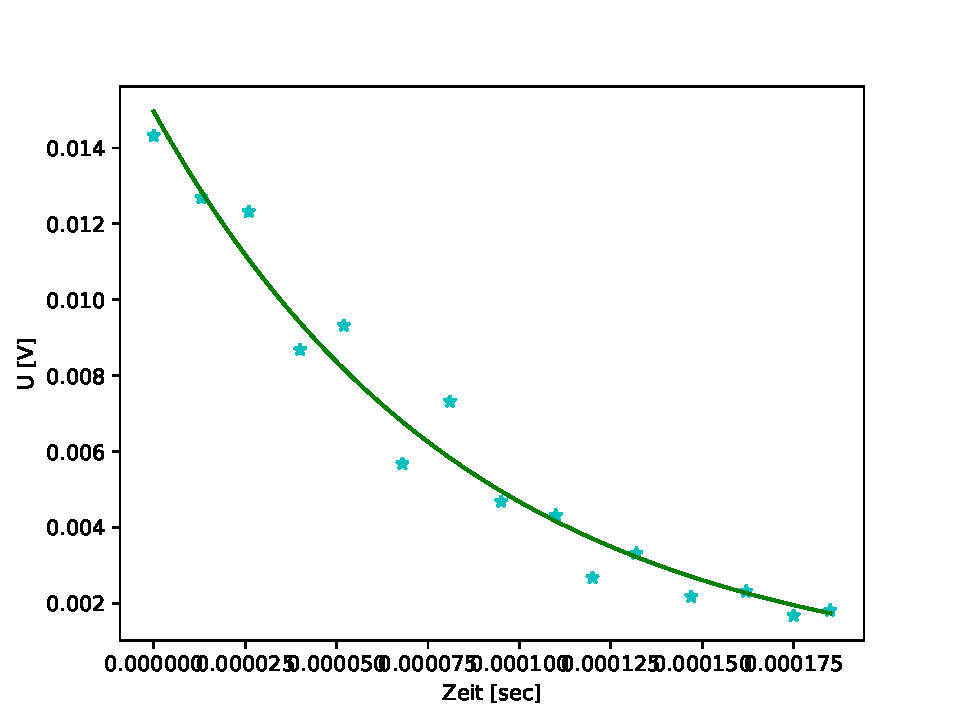
\includegraphics{Python/plot1.pdf}
    \caption{Plot.}
    \label{fig:plot}
  \end{figure}
  Mit der Funktion $U=U_0\cdot e^{-2 \pi \mu t}$ wird eine Ausgleichsrechnung durchgeführt.
  Dabei ergeben sich folgende Regressionsparameter:
  \begin{align*}
    U_0=0.015\pm 0.001 V\\
    \mu = 1849.3 \pm 119.03 \dfrac{1}{s}
  \end{align*}
  Aus $\mu$ lassen sich mittels 
  \begin{equation*}
    R_{eff}=4 \pi L \mu = 297 \pm 19 \SI{1}{\ohm}
  \end{equation*}
  der effektive Wiederstand und die Abklingdauer
  \begin{equation*}
    T_{ex}=\dfrac{1}{2\pi \mu} = (8.6 \pm 0.6)\cdot 10^{-5} s
  \end{equation*}
  berechnen. Die Fehler wurden mittels numpy bestimmt.

\subsection{Bestimmung des Dämpfungswiederstandes beim aperiodischen Grenzfall}
  Der aperiodische Grenzfall tritt bei dem Dämpfungswiederstand 
  \begin{align*}
    R_{ap}=1300 \SI{1}{\ohm}
  \end{align*}
  ein. Der theoretische Wert lautet
  \begin{align*}
    R=2 \sqrt{\dfrac{L}{C}}=4974\pm19 \SI{1}{\ohm}.
  \end{align*}

\subsection{Frequenzabhängigkeit der Kondensatorspannung}
  Die gemessene Kondensatorspannung und zugehörige Frequenz f bei der Erregerspannung
  $U_0 = 50 Hz$ sind in der folgenden Tabelle aufgeführt.
  \begin{table}[H]
    \centering
    \caption{Gemessene Kondensatorspannungen}
    \label{tab:data}
    \begin{tabular}{c c}
      \toprule
      Kondesatorspannung [V] & Frequenz [kHz] \\
      \midrule
      5   & 50 \\
      7.5 & 45 \\
      10  & 42 \\
      12.5& 38 \\
      12.5& 36 \\
      12.5& 34 \\
      10.5& 30 \\
      8   & 26 \\
      \bottomrule
    \end{tabular}
  \end{table}
  In Abbildung \ref{fig:plot2} sind die Werte grafisch dargestellt. 
  \begin{figure}
    \centering
    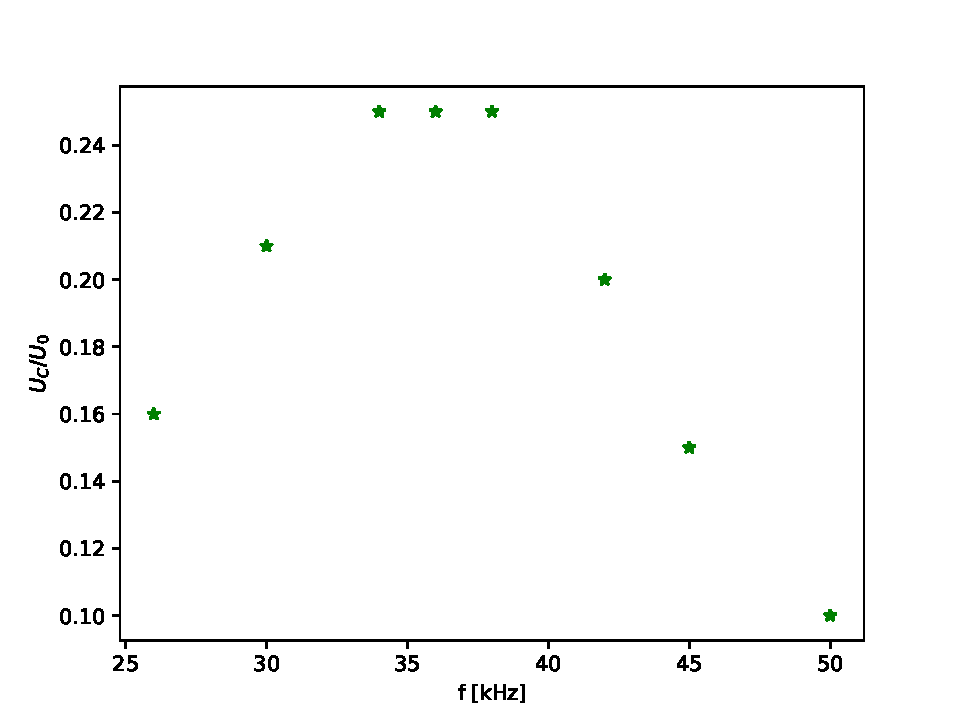
\includegraphics{Python/plot2.pdf}
    \caption{Resonanzkurve}
    \label{fig:plot2}
  \end{figure}
  Die Breite der Resonanzkurve kann aus den gemessenen Daten nicht bestimmt werden.
  Das Maximum liegt bei 36 kHz. 
